\begin{remark}
    Section made from lectures done by Kjellmar Oksavik. Other sources are \citet{BrekkeAsgeir2013Potu} --- chapter 5 parts 1 to 4 \& chapter 6 parts 1 and 6.
\end{remark}
\section{The steady-state approach}
We start with the momentum equation for an ion species \(j\)
\begin{equation*}
    \rho_j\fracd{\gf{v}_j}=-\nabla p_j+\rho_j\gf{g}+\frac{q_j\rho_j}{m_j}\left(\gf{E}+\gf{v}_j\times\gf{B}\right)-\sum_{\substack{k\\ j\neq k}}\rho_{j}v_{jk}\left(\gf{v}_j-\gf{v}_k\right)
\end{equation*}
Usually, it is also assumed that the number density of positive ions is set equal to the number density of electrons, thus
\begin{equation*}
    n_e=n_i=\sum_{\tn{ions}}n_j
\end{equation*}
Due to the coupling this may turn out to be very complex. In order to understand the basic features of ionospheric dynamics it is therefore more practical to consider a single ion species of mass \(m_i\) or, equivalently, assume a pseudo-ion derived by proper weighting of all ions with respect to their individual mass, density, charge, velocity and temperature. Neglecting the pressure and gravity terms, the momentum equation for ions and electrons can respectively be expressed as
\begin{align*}
    n_{i}m_i\fracd{\gf{v}_i}=n_{i}e\left(\gf{E}+\gf{v}_i\times\gf{B}\right)-n_{i}m_i\nu_{in}\left(\gf{v}_i-\gf{u}_n\right)\\
    n_{e}m_e\fracd{\gf{v}_e}=-n_{e}e\left(\gf{E}+\gf{v}_e\times\gf{B}\right)-n_{e}m_e\nu_{en}\left(\gf{v}_e-\gf{u}_n\right)
\end{align*}

An approximate formula for electron collision frequency is
\begin{equation*}
    \nu_e\equiv \nu_{en}+\nu_{ei}=\num{5.4e-10}n_{n}T_e^{1/2}+\left[34+4.18\ln\left(\frac{T_e^3}{n_e}\right)\right]n_{e}T_e^{-3/2}
\end{equation*}
The densities are given in \(\tn{cm}^{-3}\).

When we compare the terms including velocities in the momentum equation, we find that the acceleration term on the left-hand side is of the order \(v_j/\tau_j\) or \(v_j^2/L\), where \(\tau_j\) is the response time and \(L\) is a distance characteristic for velocity change. The Lorentz term on the right-hand side is of the order of \(\nu_j\Omega_j\), where \(\Omega_j\) is the gyrofrequency (\(q_{j}B/m_j\)) for ion species \(j\), and the frictional term is of order \(\nu_{jk}\) where \(\nu_{jk}\) is the collision frequency. As long as \(\tau_j\gg \Omega_j^{-1}\)or \(\tau_j\gg \nu_j^{-1}\) the inertia term can be neglected. The collision frequency and gyrofrequency are sufficiently large that in most problems of interest to macroscopic dynamics this is a valid simplification.

The stead-state solution of the ion momentum equation is
\begin{equation*}
    n_{i}e\left(\gf{E}+\gf{v}_i\times\gf{B}\right)-n_{i}m_i\nu_{in}\left(\gf{v}_i-\gf{u}_n\right)=0
\end{equation*}
and equivalently for electrons. From this we derive the ion velocity
\begin{equation*}
    \gf{v}_i=\gf{u}_n+\frac{e}{m_i\nu_{en}}\left(\gf{E}+\gf{v}_i\times\gf{B}\right)
\end{equation*}
and again for the electrons it is the same but with a change of sign for the last term. We rearrange to obtain
\begin{equation*}
    \gf{v}_i'=\frac{e}{m_i\nu_{in}}\gf{E}'+\frac{e}{m_i\nu_{in}}\gf{v}_i'\times\gf{B},\qquad\gf{E}'=\gf{E}+\gf{u}_n\times\gf{B}, \gf{v}_i'=\gf{v}_i-\gf{u}_n
\end{equation*}
Changing the sign gives the same equation for electrons.

Let us now assume that the neutral wind can be neglected, hence
\begin{equation}\label{eq:L12_equation_for_v_i}
    \gf{v}_i=\frac{k_i}{B}\gf{E}+\frac{k_i}{B}\gf{v}_i\times\gf{B}
\end{equation}
where \(k_i=\Omega_i/\nu_{in}\) is the ion mobility coefficient when \(\Omega_i=eB/m_i\). We take the cross product with the magnetic field, yielding
\begin{equation*}
    \gf{v}_i\times\gf{B}=\frac{k_i}{B}\gf{E}\times\gf{B}+\frac{k_i}{B}\left(\gf{v}_i\cdot\gf{B}\right)\gf{B}-k_{i}B\gf{v}_i
\end{equation*}
and
\begin{equation*}
    \gf{v}_i\cdot\gf{B}=\frac{k_i}{B}\gf{E}\cdot\gf{B}
\end{equation*}
we combine to two last equations and plug this into \cref{eq:L12_equation_for_v_i} which gives us
\begin{equation*}
    \gf{v}_i=\frac{k_i}{B}\gf{E}+{\left(\frac{k_i}{B}\right)}^2\gf{E}\times\gf{B}+{\left(\frac{k_i}{B}\right)}^3\left(\gf{E}\cdot\gf{B}\right)\gf{B}-k_i^2\gf{v}_i
\end{equation*}
Solving this for \(\gf{v}_i\) yields
\coloredeq{eq:L12_v_i_equation_big}{
    \gf{v}_i=\frac{1}{1+k_i^2}\left[\frac{k_i}{B}\gf{E}+\left(\frac{k_i}{B}\right)^2\gf{E}\times\gf{B}+\left(\frac{k_i}{B}\right)^3\left(\gf{E}\cdot\gf{B}\right)\gf{B}\right]
}
The first term in the bracket is along the \(E\)-field, the second perpendicular to both the \(E\)- and \(B\)-field, while the last term is along the \(B\)-field. The equivalent equation for electrons is the same, but with a change in sign on the first and third term in the bracket.

Allowing the neutral wind to be nonzero, we can replace \(\gf{v}_i,\gf{v}_e\) and \(\gf{E}\) by \(\gf{v}_i',\gf{v}_e'\) and \(\gf{E}'\). This gives us
\begin{equation*}
    \gf{v}_i'=\gf{v}_i-\gf{u}_n=\frac{1}{1+k_i^2}\left[\frac{k_i}{B}\gf{E}'+{\left(\frac{k_i}{B}\right)}^2\gf{E}'\times\gf{B}+{\left(\frac{k_i}{B}\right)}^3\left(\gf{E}'\cdot\gf{B}\right)\gf{B}\right]
\end{equation*}
which is the exact same thing except from the primes. I.e.\ we only change the values of the electric field.
\begin{figure}[t]
    \centering
    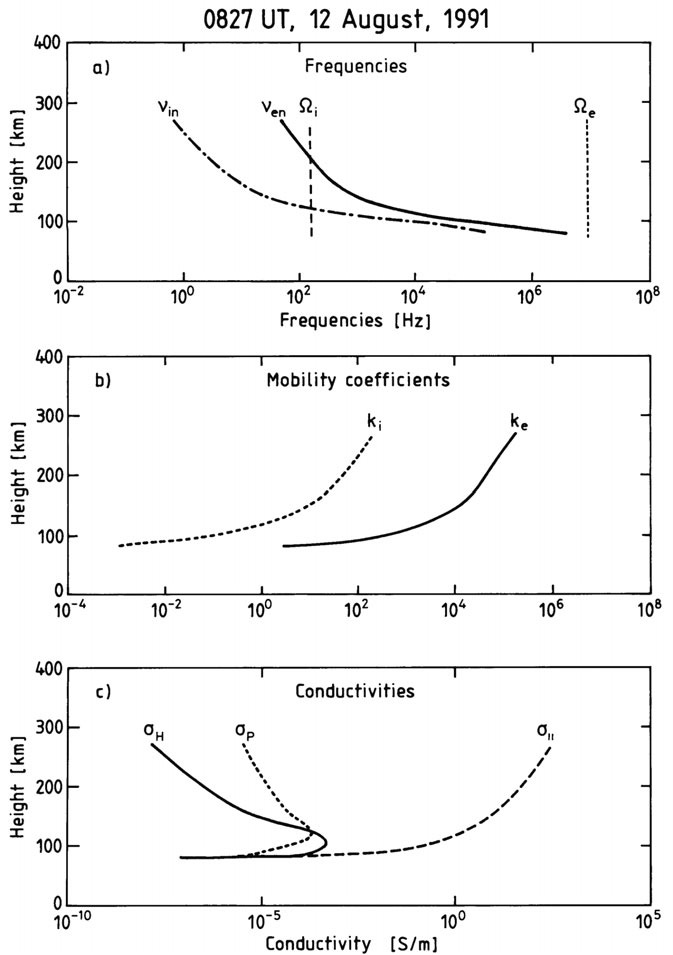
\includegraphics[width=.6\linewidth]{bilder/L12_k_i_for_ion_and_electron.jpg}
    \caption{(a) Typical altitude profiles of ion-neutral (\(\nu_{in}\)) and electron–neutral (\(\nu_{en}\)) collision frequencies for an auroral zone station such as Tromsø (69\si{\degree}39' N, 18\si{\degree}56' E). Also indicated for comparison are the ion (\(\Omega_i\)) and electron (\(\Omega_e\)) gyrofrequencies. (b) Altitude profiles of the ion (\(k_i=\Omega_i/\nu_{in}\)) and electron mobility coefficients derived from the profiles given in panel (a). (c) Altitude profiles of the Pedersen (\(\sigma_P\)), Hall (\(\sigma_H\)), and parallel (\(\sigma_{||}\)) conductivities as derived by EISCAT at Tromsø at 08:27 UT on August 12, 1991. These profiles are typical of quiet summer days. (Courtesy Blixt, 1995.)}\label{fig:L12_k_i_for_ion_and_electron}
\end{figure}

\section{Dependence of ion velocity direction on altitude}
We look back at a previous result, where we found an expression for the ion and electron velocity given on the form as in \cref{eq:L12_v_i_equation_big}.

We now neglect all other forces except the electrostatic field \(\gf{E}\) for a while and assume \(\gf{E}\cdot\gf{B}=0\). \Cref{eq:L12_v_i_equation_big} will then look like
\begin{equation*}
    \gf{v}_i=\frac{k_i}{1+k_i^2}\frac{\gf{E}_\perp}{B}+\frac{k_i^2}{1+k_i^2}\frac{\gf{E}_\perp\times\gf{B}}{B^2}
\end{equation*}
with a change of sign on the first term giving the same equation for electrons.

In the F-region we have that \(\nu_{in}\ll\Omega_i\Rightarrow k_i\gg 1\) which then imply
\begin{equation*}
    \gf{v}_i\approx\frac{\gf{E}_\perp\times\gf{B}}{B^2}
\end{equation*}
i.e.\ the ions \(\gf{E}\times\gf{B}\)-drift.

In the D-region the opposite is the case, \(\nu_{in}\gg\Omega_i\Rightarrow k_i\ll 1\) which imply
\begin{equation*}
    \gf{v}_i\approx k_i\frac{\gf{E}_\perp}{B}
\end{equation*}
We introduce an angle \(\theta_i\) to denote the angle between the electric field and the ion velocity. This will be given as
\begin{equation*}
    \tan\theta_i=k_i=\frac{\Omega_i}{\nu_{in}}
\end{equation*}
Therefore, in the F-region we have \(\theta_{i,\tn{F-region}}=\SI{90}{\degree}\), at 125 km altitude where the collision frequency is about the same as the gyro frequency we have \(\theta_{i,\tn{125 km}}=\SI{45}{\degree}\) and in the D-region we have \(\theta_{i,\tn{D-region}}=\SI{0}{\degree}\). As we can observe ion velocities in the ionosphere by incoherent scatter radar experiments, we can derive at different heights the angle between the electric field and the ion velocity. If this angle does not agree with the angle \(\theta_i\) derived above, we can infer that there must have been a neutral wind present.

The magnitude of the ion velocity is
\begin{equation*}
    v_i=k_i{\left(1+k_i^2\right)}^{-1/2}\frac{E}{B}=\sin\theta_i\frac{E}{B}
\end{equation*}
From this we see that in the D-region the ion velocity goes to zero (\(\theta_i\approx\SI{0}{\degree}\)) due to the high number of collisions. In the F-region, upper ionosphere, where \(\theta_i\approx\SI{90}{\degree}\) we get that \(v_i\approx E/B\).

The same can be done for electrons, and it can be shown that
\begin{equation*}
    \tan\theta_e=-k_e=-\frac{\Omega_e}{\nu_{en}}
\end{equation*}
with a magnitude of
\begin{equation*}
    v_e=k_e{\left(1+k_e^2\right)}^{-1/2}\frac{E}{B}=-\sin\theta_e\frac{E}{B}
\end{equation*}
The different directions of the velocities at different heights is illustrated in \cref{fig:L14_v_i_v_e_electric_field}.
\begin{figure}[t]
    \centering
    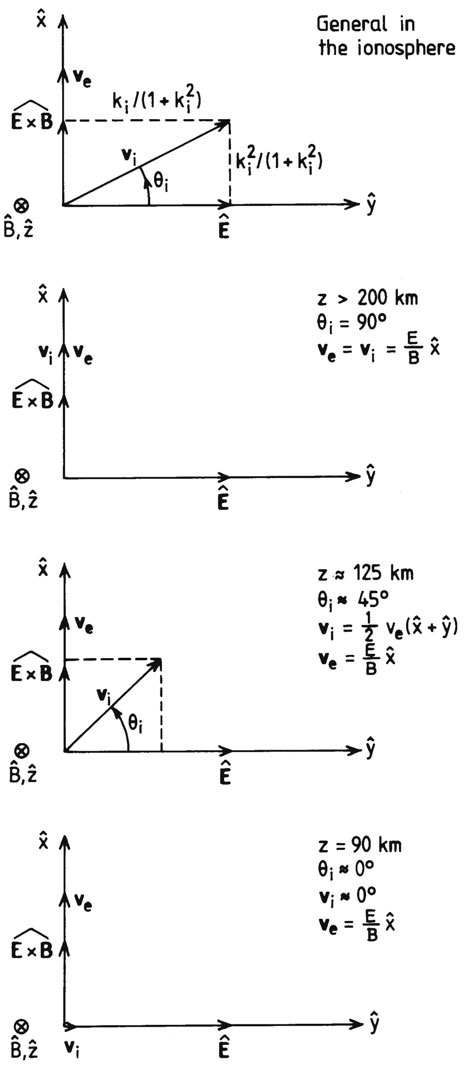
\includegraphics[width=.4\linewidth]{bilder/L14_v_i_v_e_electric_field.jpg}
    \caption{Vector diagrams showing the variation of \(v_i\) and \(v_e\) in the applied electric field for three different altitudes in the ionosphere.}\label{fig:L14_v_i_v_e_electric_field}
\end{figure}
The rotation of the ion velocity with respect to the electric field and the electron velocity in the ionosphere is, as we have demonstrated above, a result of varying collision frequency with height.

\section{Current density in the ionosphere}
We write out the current with the expressions for \(\gf{v}_i\) and \(\gf{v}_e\) we found in \cref{eq:L12_v_i_equation_big}. This yields
\begin{align}
    \gf{j}&=n_{e}e\left \{\left(\frac{k_e}{1+k_e^2}+\frac{k_i}{1+k_i^2}\right)\frac{\gf{E}_\perp}{B}-\left(\frac{k_e^2}{1+k_e^2}-\frac{k_i^2}{1+k_i^2}\right)\frac{\gf{E}\times\gf{B}}{B^2}+\left(k_e+k_i\right)\frac{\gf{E}_{||}}{B}\right \}\notag \\
    &=\sigma_P\gf{E}_\perp-\sigma_H\frac{\gf{E}\times\gf{B}}{B}+\sigma_{||}\gf{E}_{||}\label{eq:L14_current_equation}
\end{align}
where we have used the conductivities
\begin{align*}
    \sigma_P&=\frac{n_{e}e}{B}\left(\frac{k_e}{1+k_e^2}+\frac{k_i}{1+k_i^2}\right)\\
    \sigma_H&=\frac{n_{e}e}{B}\left(\frac{k_e^2}{1+k_e^2}-\frac{k_i^2}{1+k_i^2}\right)\\
    \sigma_{||}&=\frac{n_{e}e}{B}\left(k_e+k_i\right)\\
\end{align*}

We notice in \cref{fig:L14_three_currents} that while the maximum Pedersen conductivity is approximately determined by height where \(\Omega_i=\nu_{in}\), the maximum Hall conductivity is more closely related to the peak in the electron density profile. For this reason the Hall conductivity is more sensitive to high-energy auroral particle precipitation, which enhances ionization below 125 km very strongly.
\begin{figure}[t]
    \centering
    \begin{subfigure}[t]{.9\linewidth}
        \centering
        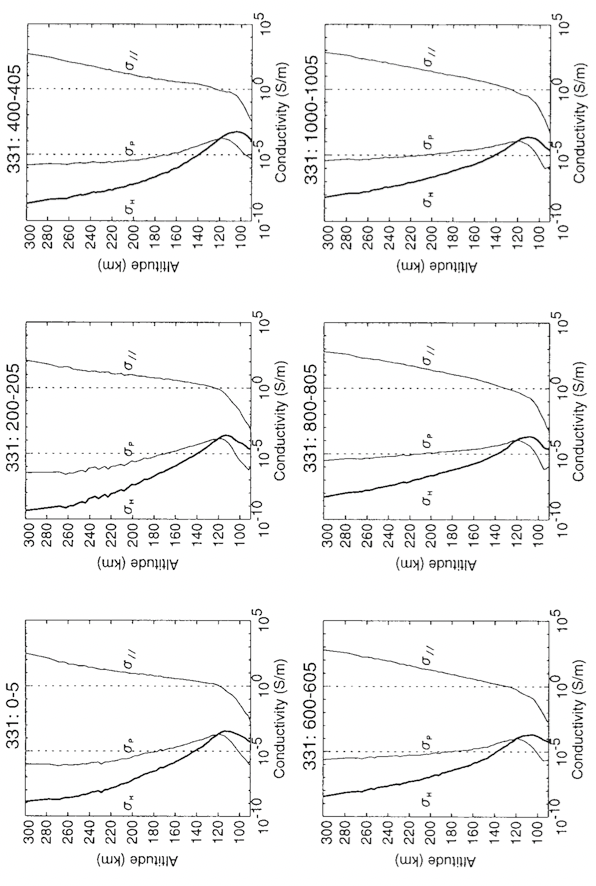
\includegraphics[width=.7\linewidth, angle=270]{bilder/L14_three_currents1.png}
        \caption{}\label{fig:L14_three_currents1}
    \end{subfigure}

    \begin{subfigure}[t]{.9\linewidth}
        \centering
        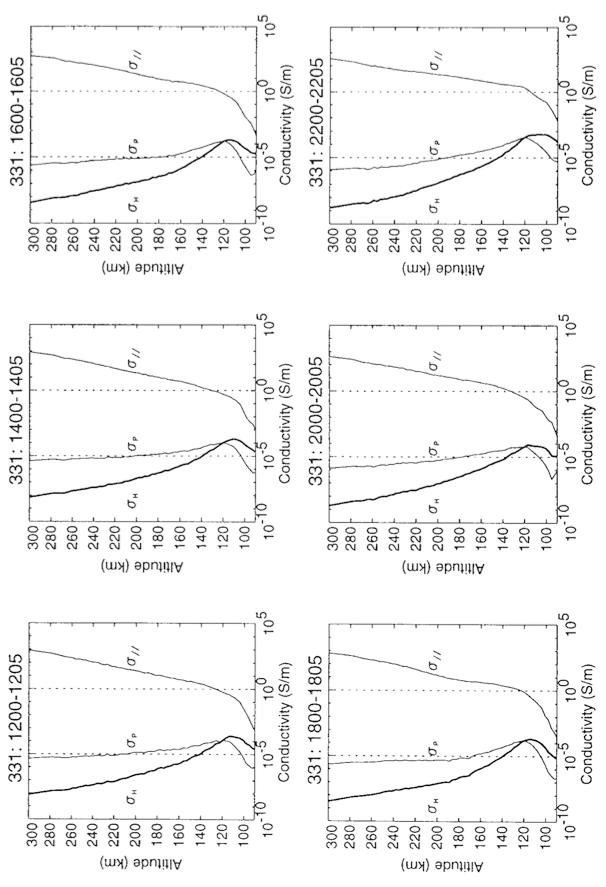
\includegraphics[width=.7\linewidth, angle=270]{bilder/L14_three_currents2.png}
        \caption{}\label{fig:L14_three_currents2}
    \end{subfigure}

    \caption{Examples of Pedersen, Hall, and parallel conductivity profiles (in siemens/m) as derived at the Tromsø auroral zone station for 12 different time intervals on 31 March, 1992. (Courtesy Nozawa, 1995.)}\label{fig:L14_three_currents}
\end{figure}

\section{Height-dependent currents and heating rates}
We now look at the Joule heat dissipation rate. The height-dependent heat dissipation rate due to current flowing along an electric field perpendicular to \(\gf{B}\) (Joule heat dissipation) is given by
\begin{equation*}
    q_J(z)=\gf{j}(z)\cdot\gf{E}=(\sigma_P(z)\gf{E}_\perp-\sigma_H(z)\gf{E}_\perp\times\gf{B}/B)\cdot\gf{E}_\perp=\sigma_P(z)E_\perp^2
\end{equation*}
If we rewrite this in the neutral wind frame of reference, we get
\begin{equation*}
    q_J'(z)=\sigma_P(z){\gf{E}_\perp'}^2=\sigma_P(z){\left(\gf{E}_\perp+\gf{u}_n(z)\times\gf{B}\right)}^2
\end{equation*}
We see that \(\sigma_H\) does not contribute to the heat dissipation. If \(\gf{E}_\perp+\gf{u}_n(z)\times\gf{B}=0\) then there are no Joule heating.

The magnitude of the current density at height \(z\) is
\begin{equation*}
    j{(z)}_\perp=\frac{e}{B}\frac{1}{\sqrt{1+k_i^2}}n_e(z)E_\perp'=\frac{e}{B}\frac{1}{\sqrt{1+k_i^2}}n_e(z)\left|\gf{E}_\perp+\gf{u}_n(z)\times\gf{B}\right|
\end{equation*}
The neutral wind is a very elusive parameter and extremely difficult to measure simultaneously at different altitudes for considerable lengths of time. This makes the neutral wind extra complicated to implement in models, and some averaging assumptions usually have to be made.

We can write up the Joule heating dissipation on another form, in the reference frame of the neutral wind, as
\begin{equation*}
    q_J'(z)=\gf{j}'(z)\cdot\gf{E}_\perp'(z)=\left(\sigma_P(z)\cdot\gf{E}_\perp'(z)-\sigma_H(z)\frac{\gf{E}_\perp'(z)\times\gf{B}}{B}\right)\cdot\gf{E}_\perp'(z)=\sigma(z){\left(\gf{E}_\perp'(z)\right)}^2\geq 0
\end{equation*}
or
\begin{equation*}
    q_J'(z)=\gf{j}'(z)\cdot\left(\gf{E}_\perp+\gf{u}_n(z)\times\gf{B}\right)=\gf{j}'(z)\cdot\gf{E}_\perp-\left(\gf{j}'(z)\times\gf{B}\right)\cdot\gf{u}_n(z)\geq 0
\end{equation*}

\section{Mapping of \(E\)-fields in the ionosphere}
We start by assuming finite conductivity \(\perp\gf{B}\), implying that electric fields are not necessarily conserved. Our coordinate system is defined by the vertical magnetic field being \(\gf{\widehat{B}}=-\f{z}\). The electric field is given by \(\gf{E}=E_x\f{x}+E_y\f{y}+E_z\f{z}\) and the current is given by \cref{eq:L14_current_equation} which we rewrite as
\begin{equation*}
    \gf{j}(z)=\left(\sigma_{P}E_x+\sigma_{H}E_y\right)\f{x}+\left(\sigma_{P}E_y-\sigma_{H}E_x\right)\f{y}+\sigma_{||}E_z\f{z}
\end{equation*}
This may be written up on tensor form as
\begin{equation*}
    \left(\begin{array}{c}
        j_x\\j_y\\j_z
    \end{array}\right)=\left(\begin{array}{ccc}
        \sigma_P & \sigma_H & 0\\
        -\sigma_H & \sigma_P & 0\\
        0 & 0 & \sigma_{||}
    \end{array}\right)\cdot
    \left(\begin{array}{c}
        E_x\\E_y\\E_z
    \end{array}\right)\Leftrightarrow\gf{j}=\widetilde{\sigma}\cdot\gf{E}
\end{equation*}

We now assume that conductivities are functions of \(z\) only. Since the current must be divergence free we find
\begin{equation*}
    \nabla\cdot\gf{j}=\sigma_P\p{x}{E_x}+\sigma_H\p{x}{E_y}+\sigma_P\p{y}{E_y}-\sigma_H\p{y}{E_x}+\p{z}{\left(\sigma_{||}E_z\right)}=0
\end{equation*}
Taking advantage of \(\nabla\times\gf{E}=0\) we write
\begin{equation*}
    \nabla\cdot\gf{j}=\sigma_P\left(\p{x}{E_x}+\p{y}{E_y}\right)+\p{z}{\left(\sigma_{||}E_z\right)}=0
\end{equation*}
Since the electric field must be deduced from a potential as \(\gf{E}=\nabla\phi \), we obtain
\begin{equation*}
    \p{xx}{\phi}+\p{yy}{\phi}+\frac{1}{\sigma_P}\p{z}{\left(\sigma_{||}\p{z}{\phi}\right)}=0
\end{equation*}
We will now introduce the following substitution
\begin{equation*}
    \tn{d}z'=\sqrt{\frac{\sigma_P}{\sigma_{||}}}\tn{d}z \Rightarrow \p{z}{}=\sqrt{\frac{\sigma_P}{\sigma_{||}}}\p{z'}{}
\end{equation*}
If we also introduce the geometric mean \(\sigma_m=\sqrt{\sigma_P\sigma_{||}}\) we get
\begin{equation*}
    \p{xx}{\phi}+\p{yy}{\phi}+\p{z'z'}{\phi}+\frac{1}{\sigma_m}\p{z'}{\sigma_m}\p{z'}{\phi}=0
\end{equation*}
If we now assume that \(\sigma_m=\sigma_0\exp(-z'/\alpha)\) this equation will be much simplified. \(\alpha \) is here a constant scale height. This does not limit the applicability of the solutions obtained since any reasonable conductivity profile can be closely approximated by a series of simple exponential functions. Inserting the new conductivity yields
\begin{equation*}
    \p{xx}{\phi}+\p{yy}{\phi}+\p{z'z'}{\phi}-\frac{1}{\alpha}\p{z'}{\phi}=0
\end{equation*}
where this can be solved by the method of separation of variables. We will assume that the electrostatic potential is generated at a source level \(z_0'\) and that it has sinusoidal spatial variations with wavelength \(\lambda \) in both the \(x\)- and \(y\)-directions. The solution is then given by
\begin{equation*}
    \phi=\phi_0\exp\left[A\left(z'-z_0'\right)\right]\exp\left[\frac{2\pi i}{\lambda}\left(x+y\right)\right]
\end{equation*}
where \(A\) satisfies the equation
\begin{equation*}
    A^2-\frac{1}{\alpha}A-\frac{8\pi^2}{\lambda^2}=0
\end{equation*}
with roots
\begin{align*}
    A_1&=\frac{1}{2\alpha}-\sqrt{{\left(\frac{1}{2\alpha}\right)}^2+\frac{8\pi^2}{\lambda^2}}<0\\
    A_2&=\frac{1}{2\alpha}+\sqrt{{\left(\frac{1}{2\alpha}\right)}^2+\frac{8\pi^2}{\lambda^2}}>0
\end{align*}
Thus, the complete solution is
\coloredeq{eq:L14_electric_potential}{\phi=\left \{S_1\exp\left[A_1\left(z'-z_0'\right)\right]+S_2\exp\left[A_2\left(z'-z_0'\right)\right]\right \}\exp\left[\frac{2\pi{} i}{\lambda}\left(x+y\right)\right]\phi_0}
where \(S_1\) and \(S_2\) are constants to be determined by the boundary conditions of the problem. We see how the potential behave with regards to damping at different heights in \cref{fig:L14_electric_potential}.
\begin{figure}[t]
    \centering
    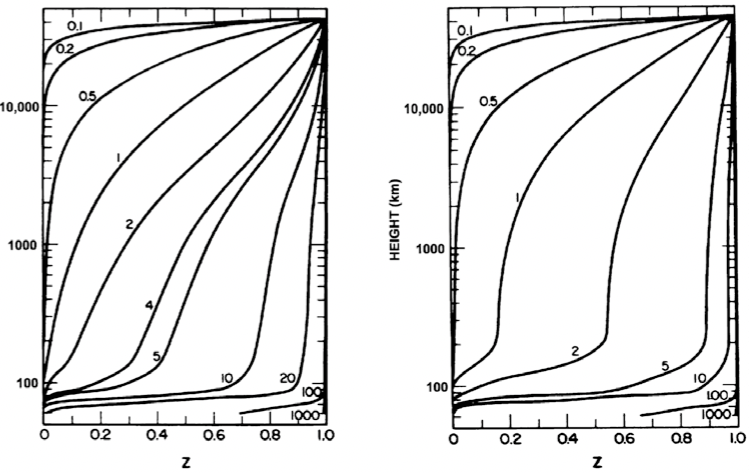
\includegraphics[width=.8\linewidth]{bilder/L14_electric_potential.png}
    \caption{(Left panel) The potential transmission factor (\(Z\)) as a function of altitude under daytime conditions. \(Z\) is the ratio between the potential at a particular altitude and at the source region. The labels on the curves refer to spatial wavelength (\(\lambda \)) in kilometers. (Right panel) The potential transmission factor (\(Z\)) as a function of altitude under night-time conditions. (From Reid, 1965.)}\label{fig:L14_electric_potential}
\end{figure}